\documentclass{CSICC}

\usepackage{booktabs}
\usepackage{array}
\usepackage{siunitx}
\usepackage{multirow}
\usepackage{amsmath}
\usepackage{graphicx}
\usepackage{float}

\title{
تخمین تحرک در شبکه‌های 4G LTE با استفاده از یادگیری ماشین
}

\author[1]{فاطمه اسماعیلی}
\author[2]{علی رحیم‌زاده}
\author[3]{شادی زرگرزاده}

\affil{
دانشگاه علم و صنعت ایران، دانشکده مهندسی کامپیوتر،\\
\lr{esmaeli@comp.iust.ac.ir},
\lr{rahimzadeh@comp.iust.ac.ir},
\lr{alizargar@comp.iust.ac.ir}
}

\date{ژانویه 2026}

\begin{document}
\maketitle
\begin{abstract}
این مقاله یک رویکرد یادگیری ماشین برای تخمین سرعت و شتاب کاربر بر اساس معیارهای کیفیت سیگنال در شبکه‌های موبایل نسل چهارم \lr{(4G)} ارائه می‌دهد. ما از رابطه بین تحرک کاربر و ویژگی‌های سیگنال سلولی، از جمله توان سیگنال مرجع دریافتی \lr{(RSRP)}، کیفیت سیگنال مرجع دریافتی \lr{(RSRQ)} و نسبت سیگنال به تداخل به علاوه نویز \lr{(SINR)} استفاده می‌کنیم. از طریق اصلاح تکراری مدل، نشان می‌دهیم که الگوریتم‌های جنگل تصادفی و تقویت گرادیان می‌توانند پارامترهای حرکت کاربر را با دقت پیش‌بینی کنند. مدل نهایی ما به امتیاز \(R^{2}\) برابر با 916.0 برای تخمین سرعت و 907.0 برای تخمین شتاب، با میانگین خطای مطلق 594.0 متر بر ثانیه و 38.0 متر بر ثانیه مربع به ترتیب دست می‌یابد.
\end{abstract}

\begin{keywords}
تخمین تحرک کاربر، شبکه‌های \lr{4G}، یادگیری ماشین، جنگل تصادفی، تقویت گرادیان، معیارهای کیفیت سیگنال
\end{keywords}

\section{مقدمه}

\subsection{پیشینه و انگیزه}
با استقرار فراگیر شبکه‌های نسل چهارم \lr{(4G)} تکامل بلندمدت، توانایی استخراج هوش ثانویه از تله‌متری استاندارد شبکه به حوزه مهمی از تحقیقات تبدیل شده است. تخمین دقیق تحرک کاربر به طور خاص سرعت و شتاب یک نیاز اساسی برای نسل بعدی مدیریت هوشمند شبکه است.

محرک‌های اصلی برای توسعه تخمین تحرک مبتنی بر سیگنال شامل موارد زیر است:

\textbf{بهینه‌سازی منابع شبکه:} تخصیص پویای منابع و مدیریت پیشگیرانه تحویل به پیش‌بینی زمانی که تجهیزات کاربری \lr{(UE)} بین سلول‌ها جابجا می‌شود، وابسته است. تخمین دقیق سرعت اثرات "پینگ‌پنگ" و سربار سیگنال‌دهی را کاهش می‌دهد.

\textbf{سرویس‌های مبتنی بر مکان \lr{(LBS)}:} \lr{LBS} سنتی به شدت به سیستم‌های ناوبری ماهواره‌ای جهانی \lr{(GNSS)} وابسته است. با این حال، \lr{GNSS} به طور بدنامی انرژی‌بر است و از تخریب سیگنال در "دره‌های شهری" یا محیط‌های داخلی رنج می‌برد.

\textbf{سیستم‌های حمل‌ونقل هوشمند \lr{(ITS)}:} نظارت بر ترافیک بلادرنگ و ردیابی سرعت وسایل نقلیه می‌تواند با داده‌های سلولی تقویت شود و یک مکانیسم ایمن برای خودروهای خودران و متصل فراهم کند.

علی‌رغم دقت \lr{GPS}، مصرف انرژی بالا و حساسیت آن به مسدودسازی‌های محیطی، نیاز به یک رویکرد جایگزین را ضروری می‌سازد. استفاده از معیارهای صفحه کنترل \lr{4G} موجود یک پارادایم سنجش "صفر-هزینه" ارائه می‌دهد که از سیگنال‌هایی که قبلاً توسط \lr{UE} برای اتصال استاندارد اندازه‌گیری می‌شوند، استفاده می‌کند.

\subsection{بیان مسئله}
چالش اصلی که در این تحقیق مورد توجه قرار گرفته است، \textit{مسئله نگاشت غیرخطی} بین معیارهای فرکانس رادیویی \lr{(RF)} و سینماتیک فیزیکی است. هدف ما تخمین سرعت لحظه‌ای \((v)\) و شتاب \((a)\) یک \lr{UE} با استفاده از یک بردار ویژگی \(\mathbf{X}\) است که منحصراً از سه شاخص کیفیت سیگنال استخراج شده است: توان سیگنال مرجع دریافتی \lr{(RSRP)}، کیفیت سیگنال مرجع دریافتی \lr{(RSRQ)} و نسبت سیگنال به تداخل به علاوه نویز \lr{(SINR)}.

از نظر ریاضی، هدف بهینه‌سازی یک تابع رگرسیون \(f\) است به طوری که:

\[
(v,a)\approx f(\text{\lr{RSRP}},\text{\lr{RSRQ}},\text{\lr{SINR}})
\]

در حالی که مختصات \lr{GPS} در طول مرحله آموزش برای ایجاد برچسب‌های واقعیت زمینی استفاده می‌شود، مدل استنتاج پیشنهادی کاملاً مستقل از \lr{GPS} باقی می‌ماند و عملکرد کم‌مصرف را در استقرارهای دنیای واقعی تضمین می‌کند.

\subsection{مشارکت‌های پیشنهادی}
این کار به طور سیستماتیک امکان‌سنجی تخمین حرکت مبتنی بر سیگنال را از طریق یک فرآیند توسعه تکراری بررسی می‌کند. مشارکت‌های کلیدی به شرح زیر خلاصه می‌شوند:

\begin{enumerate}
\item \textbf{خط لوله تکراری یادگیری ماشین:} ما یک چارچوب توسعه چند مرحله‌ای را پیشنهاد می‌کنیم که از رگرسیون پایه به مدل‌های پیچیده تقویت‌شده گرادیان تکامل می‌یابد و به طور خاص واریانس بالا در داده‌های شتاب را مورد توجه قرار می‌دهد.

\item \textbf{مهندسی ویژگی زمانی:} ما یک مجموعه ویژگی جامع شامل آمار غلتان (میانگین‌های متحرک، نوسان) و ویژگی‌های دیفرانسیلی (تغییرات سیگنال مرتبه اول و دوم) را برای به دست آوردن دینامیک زمانی حرکت معرفی می‌کنیم.

\item \textbf{تحلیل الگوریتمی مقایسه‌ای:} یک ارزیابی عملکرد دقیق بین الگوریتم‌های جنگل تصادفی و تقویت گرادیان ارائه شده است که توانایی برتر گروه‌های متوالی را در به حداقل رساندن باقیمانده‌ها در مجموعه داده‌های تحرک غیرخطی برجسته می‌کند.

\item \textbf{نتایج با وفاداری بالا:} مدل نهایی ما به ضریب تعیین \((R^{2})\) بیش از 916.0 برای سرعت و 907.0 برای شتاب دست می‌یابد و معیار جدیدی را برای تخمین مبتنی بر سیگنال با استفاده از مجموعه داده \lr{SRFG-v1} ایجاد می‌کند.
\end{enumerate}
\section{چارچوب نظری و مقدمات}

\subsection{معماری سیستم: شبکه‌های \lr{4G LTE}}
استاندارد نسل چهارم تکامل بلندمدت \lr{(4G LTE)} نشان‌دهنده یک انتقال به یک معماری تخت، تمام \lr{IP} سوئیچ‌شده بسته است که به عنوان سیستم بسته تکامل‌یافته \lr{(EPS)} شناخته می‌شود. این معماری برای به حداقل رساندن تأخیر و به حداکثر رساندن توان عبوری طراحی شده است و عملیات را به دو بخش اصلی تقسیم می‌کند:

\textbf{\lr{E-UTRAN} (شبکه دسترسی رادیویی زمینی \lr{UMTS} تکامل‌یافته):} متشکل از \lr{eNodeB}ها (\lr{Node B}های تکامل‌یافته) که به عنوان ایستگاه‌های پایه هوشمند عمل می‌کنند. برخلاف معماری‌های قدیمی، \lr{eNodeB} کنترل منبع رادیویی \lr{(RRC)}، فشرده‌سازی سرآیند و تصمیمات تحویل را به صورت محلی در لبه شبکه مدیریت می‌کند.

\textbf{\lr{EPC} (هسته بسته تکامل‌یافته):} ستون فقرات متمرکز مسئول مدیریت سطح بالا. اجزای کلیدی شامل \lr{MME} (\lr{Mobility Management Entity}) برای سیگنال‌دهی و ردیابی، و \lr{S-GW} (\lr{Serving Gateway}) برای مسیریابی بسته‌های داده کاربر است.

\begin{figure}[H]
    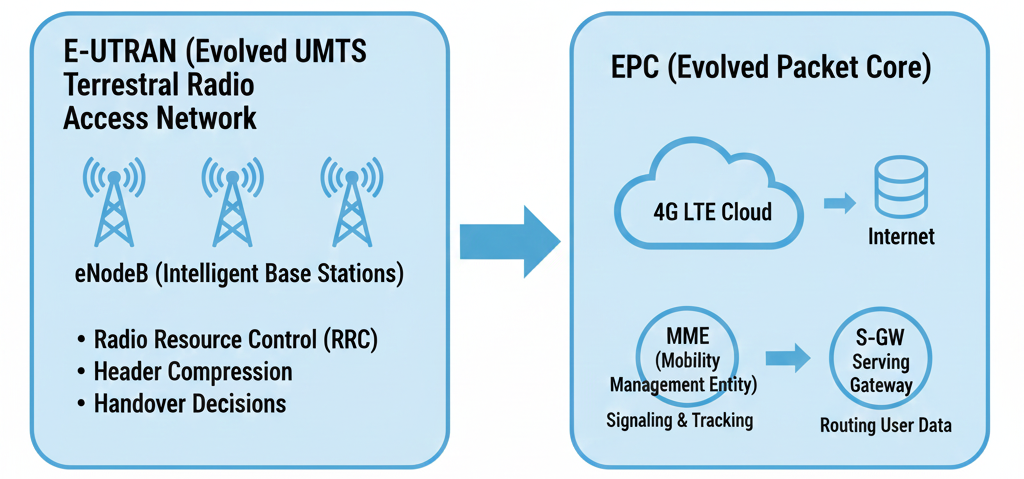
\includegraphics[width=\columnwidth]{4g_lte_architecture.png}
    \centering
    \caption{نمای کلی اجزای شبکه \lr{4G LTE} و جریان داده}
    \label{fig:4g_lte_architecture}
\end{figure}

\subsection{معیارهای عملکرد فرکانس رادیویی \lr{(RF)}}
در \lr{LTE}، تجهیزات کاربری \lr{(UE)} به طور دوره‌ای سیگنال‌های مرجع خاص سلول \lr{(CRS)} را ارزیابی می‌کند تا شرایط کانال را به شبکه گزارش دهد. مدل‌های تخمین ما از سه معیار اساسی \lr{3GPP} استفاده می‌کنند:

\subsubsection{توان سیگنال مرجع دریافتی \lr{(RSRP)}}
\lr{RSRP} به عنوان میانگین خطی مشارکت‌های توان (به وات) عناصر منبع که سیگنال‌های مرجع خاص سلول را در پهنای باند فرکانس اندازه‌گیری در نظر گرفته شده حمل می‌کنند، تعریف می‌شود.

\[
RSRP \in [-140,-44]\ \text{dBm}
\]

\lr{RSRP} معیار اصلی برای انتخاب سلول و تحویل است. در زمینه ما، به عنوان نماینده‌ای برای فاصله اقلیدسی بین \lr{UE} و \lr{eNodeB} عمل می‌کند، هرچند که تحت تأثیر محو شدن در مقیاس بزرگ است.

\subsubsection{کیفیت سیگنال مرجع دریافتی \lr{(RSRQ)}}
در حالی که \lr{RSRP} قدرت را اندازه می‌گیرد، \lr{RSRQ} نشانگری از کیفیت سیگنال با در نظر گرفتن تداخل و نویز حرارتی فراهم می‌کند. از نظر ریاضی به صورت زیر تعریف می‌شود:

\[
RSRQ=N\times\frac{RSRP}{RSSI}
\]

که در آن \(N\) تعداد بلوک‌های منبع \lr{(RB)} در پهنای باند اندازه‌گیری \lr{RSSI} (شاخص قدرت سیگنال دریافتی) است. \lr{RSRQ} به طور خاص به بار شبکه و تداخل بین سلولی حساس است.

\subsubsection{نسبت سیگنال به تداخل به علاوه نویز \lr{(SINR)}}
\lr{SINR} دقیق‌ترین شاخص پتانسیل توان عبوری کانال است. نسبت توان سیگنال مورد نظر به مجموع تمام تداخل و نویز را نشان می‌دهد:

\[
SINR=\frac{P_{\text{signal}}}{P_{\text{interference}}+N_{0}}
\]

که در آن \(N_{0}\) نویز سفید گاوسی افزودنی را نشان می‌دهد. مقادیر بالای \lr{SINR} با طرح‌های مدولاسیون مرتبه بالاتر و در نتیجه نرخ داده بالاتر همبستگی دارد.

\subsection{دینامیک تحرک و انتشار سیگنال}
حرکت یک \lr{UE} تغییرات قطعی و تصادفی را در محیط رادیویی معرفی می‌کند. این امضاهای فیزیکی اساس رویکرد یادگیری ماشین ما را تشکیل می‌دهند.

\subsubsection{تلفات مسیر و محو شدن سایه}
همانطور که یک \lr{UE} حرکت می‌کند، محو شدن در مقیاس بزرگ توسط مدل تلفات مسیر لگاریتمی-فاصله کنترل می‌شود که تضعیف سیگنال در فاصله \(d\) را مشخص می‌کند:

\[
PL(d)=PL(d_{0})+10n\log_{10}\left(\frac{d}{d_{0}}\right)+\mathcal{X}_{\sigma}
\]

که در آن \(n\) نمای تلفات مسیر و \(\mathcal{X}_{\sigma}\) نشان‌دهنده محو شدن سایه است—یک متغیر تصادفی گاوسی  ناشی از موانع در مسیر انتشار.
\subsubsection{جابجایی فرکانس دوپلر}
تغییرات زمانی در فاز سیگنال به دلیل سرعت نسبی UE رخ می‌دهد. جابجایی دوپلر \(f_d\) به صورت زیر بیان می‌شود:

\[
f_d=\frac{v\cdot f_{0}}{c}\cos(\theta)
\]

که در آن \(c\) سرعت نور و \(\theta\) زاویه ورود است. این پدیده فیزیکی نرخ تغییر در معیارهای سیگنال را مستقیماً به سرعت فیزیکی کاربر مرتبط می‌کند.



\subsection{الگوریتم‌های یادگیری گروهی برای رگرسیون}
برای نگاشت رابطه غیرخطی بین معیارهای \lr{RF} و تحرک، از روش‌های گروهی استفاده می‌کنیم که چندین یادگیرنده ضعیف را به یک پیش‌بینی‌کننده قوی ترکیب می‌کنند.

\subsubsection{جنگل تصادفی (گروه موازی)}
\lr{Random Forest } از \lr{Bagging (Bootstrap Aggregating)} برای کاهش واریانس مدل استفاده می‌کند. یک گروه از \(B\) درخت تصمیم غیرهمبسته \(\{T_{1},\ldots,T_{B}\}\) می‌سازد. خروجی نهایی رگرسیون میانگین تمام پیش‌بینی‌های درخت فردی است:

\[
\hat{y}=\frac{1}{B}\sum_{b=1}^{B}T_{b}(x)
\]

\lr{RF} در مدیریت مجموعه‌های ویژگی با ابعاد بالا بسیار مؤثر است و به طور طبیعی در برابر نویز ذاتی در مجموعه داده‌های سیگنال سلولی مقاوم است.

\subsubsection{تقویت گرادیان (گروه متوالی)}
\lr{Gradient Boosting} درخت‌ها را به صورت متوالی می‌سازد. هر درخت جدید \(h_{m}(x)\) برای به حداقل رساندن خطای باقیمانده گروه قبلی \(F_{m-1}(x)\) با دنبال کردن گرادیان منفی تابع زیان \(L\) آموزش داده می‌شود:

\[
F_{m}(x)=F_{m-1}(x)+\eta\cdot h_{m}(x)
\]

که در آن \(\eta\) نرخ یادگیری است. این بهینه‌سازی متوالی به \lr{Gradient Boosting} اجازه می‌دهد تا وابستگی‌های زمانی ظریف در شتاب را که روش‌های موازی ممکن است نادیده بگیرند، به دست آورد.

\subsection{معیارهای ارزیابی برای تخمین حرکت}
ما دقت پیش‌بینی‌های سرعت (\(v\)) و شتاب (\(a\)) خود را با استفاده از دو معیار آماری استاندارد اندازه‌گیری می‌کنیم:

1. \textbf{میانگین خطای مطلق (\lr{MAE}):} بزرگی متوسط خطاها را در همان واحدهای متغیر هدف (\lr{m/s} یا \lr{m/s\(^2\)}) اندازه‌گیری می‌کند.

2. \textbf{ضریب تعیین (\(R^2\)):} نسبت واریانس برای یک متغیر وابسته را که توسط متغیرهای مستقل توضیح داده می‌شود، نشان می‌دهد:

\[
R^2 = 1 - \frac{\sum(y_i - \hat{y}_i)^2}{\sum(y_i - \bar{y})^2}
\]

\subsection{خلاصه: پیوند سیگنال-تحرک}
فرض اساسی این تحقیق این است که معیارهای سیگنال \lr{4G} "امضاهای رمزگذاری‌شده" مسیرهای کاربر هستند. ما فرض می‌کنیم که یک نگاشت غیرخطی \(f\) وجود دارد به طوری که:

\[
v(t) \approx f\left(\mathbf{S}(t), \nabla\mathbf{S}(t), \sigma_{\mathbf{S}}(t)\right)
\]

که در آن \(\mathbf{S}(t)\) بردار معیارهای لحظه‌ای، \(\nabla\mathbf{S}(t)\) نشان‌دهنده گرادیان زمانی (نرخ تغییر)، و \(\sigma_{\mathbf{S}}(t)\) نوسان غلتان است.


\section{کارهای مرتبط}

تخمین پارامترهای تحرک کاربر یک مسئله به خوبی تثبیت‌شده در ارتباطات بی‌سیم است که به طور سنتی از طریق مدل‌های هندسی و قطعی مورد توجه قرار گرفته است. اخیراً، تمرکز به سمت پارادایم‌های داده‌محور تغییر کرده است. این فصل تحقیقات موجود را به سه حوزه اصلی دسته‌بندی می‌کند: روش‌های تحلیلی مبتنی بر سیگنال، تکنیک‌های فیلترینگ سنتی و رویکردهای یادگیری ماشین مدرن.

\subsection{روش‌های تحلیلی مبتنی بر سیگنال}
تحقیقات اولیه در تخمین تحرک به شدت بر همبستگی بین قدرت سیگنال دریافتی (RSS) و فاصله از ایستگاه پایه متکی بود. مطالعات پیشگام از مدل تلفات مسیر لگاریتمی-فاصله برای نگاشت کاهش سیگنال به سرعت کاربر استفاده کردند. در حالی که در سناریوهای خط دید (LOS) مؤثر بودند، این روش‌ها اغلب در محیط‌های شهری به دلیل محو شدن چند مسیره و سایه‌اندازی، که نویز فرکانس بالا را به اندازه‌گیری‌های RSSI (شاخص قدرت سیگنال دریافتی) معرفی می‌کنند، شکست می‌خورند.

\subsection{فیلترینگ سنتی و مدل‌سازی تصادفی}
برای کاهش نویز ذاتی در سیگنال‌های سلولی، محققان به طور گسترده فیلترهای تصادفی را اعمال کرده‌اند. فیلتر کالمن و انواع آن، مانند فیلتر کالمن توسعه‌یافته برای ردیابی وضعیت‌های کاربر با ترکیب اندازه‌گیری‌های سیگنال با معادلات سینماتیک استفاده شده است. با این حال، این مدل‌ها نیاز به یک تعریف ریاضی صریح از محیط دارند و آن‌ها را به ماهیت پویای شبکه‌های 4G که در آن الگوهای تداخل بسیار غیرخطی هستند، کمتر قابل انطباق می‌کند.

\subsection{یادگیری ماشین در تحرک سلولی}
افزایش اخیر قدرت محاسباتی منجر به پذیرش یادگیری ماشین (ML) برای پیش‌بینی تحرک شده است.

* \textbf{مدل‌های رگرسیون:} مطالعات با موفقیت از رگرسیون بردار پشتیبان (SVR) و \(k\)-نزدیک‌ترین همسایگان (k-NN) برای تخمین سرعت از RSRP و RSRQ استفاده کرده‌اند. با این حال، این مدل‌ها اغلب با وابستگی‌های زمانی موجود در داده‌های شتاب مشکل دارند.

* \textbf{یادگیری گروهی:} ادبیات اخیر پیشنهاد می‌کند که روش‌های گروهی، مانند جنگل تصادفی، با کاهش واریانس از طریق bagging از رگرسورهای تک-مدل بهتر عمل می‌کنند. کار ما با مقایسه Bagging با تکنیک‌های Boosting متوالی بر این اساس بنا شده است.

\subsection{رویکردهای ترکیبی و یکپارچه با GPS}
بخش قابل توجهی از کارهای موجود بر سیستم‌های ترکیبی تمرکز دارد که داده‌های سلولی را با GPS یا واحدهای اندازه‌گیری اینرسی (IMU) ترکیب می‌کنند. در حالی که به دقت بالا دست می‌یابند، این سیستم‌ها توسط مصرف انرژی بالای GPS و خطای انباشته انحراف IMUها محدود می‌شوند.
\subsection{تمایز کار فعلی}
تحقیق ما وضعیت هنر فعلی را با تمرکز انحصاری بر \textbf{معیارهای کیفیت سیگنال بومی 4G} (\lr{RSRP}، \lr{RSRQ} و \lr{SINR}) برای دستیابی به یک تخمین مستقل از \lr{GPS} گسترش می‌دهد. برخلاف مطالعات قبلی که اغلب سرعت و شتاب را به عنوان معیارهای ثانویه نسبت به مکان در نظر می‌گیرند، ما یک \textbf{خط لوله اصلاح تکراری} اختصاصی ارائه می‌دهیم. با نشان دادن انتقال از \lr{Random Forest} پایه به \lr{Optimized Gradient Boosting}، ما به طور خاص چالش تخمین شتاب با دقت بالا را مورد توجه قرار می‌دهیم و به یک معیار عملکرد (\(R^{2}>0.9\)) دست می‌یابیم که به ندرت در مدل‌های فقط-سیگنال به آن دست یافته می‌شود.

\section{مجموعه داده و روش‌شناسی}
\subsection{انتخاب مجموعه داده: SRFG-v1}
پایه تجربی این تحقیق \textbf{مجموعه داده \lr{SRFG-v1}} است، یک مجموعه با وضوح بالا از تله‌متری شبکه \lr{4G LTE} دنیای واقعی. این مجموعه داده به ویژه برای تخمین تحرک مناسب است زیرا معیارهای سیگنال لایه فیزیکی را با واقعیت زمینی \lr{GPS} با دقت بالا در پروفایل‌های مختلف تحرک (\lr{pedestrian}، \lr{vehicle} و \lr{high-speed}) همگام‌سازی می‌کند.
\subsubsection{شاخص‌های فرکانس رادیویی (RF)}
فضای ویژگی از سه معیار استاندارد 3GPP اولیه که کانال پایین‌رو را مشخص می‌کنند، ساخته شده است:

\textbf{\lr{RSRP (dBm)}:} نشان‌دهنده میانگین خطی مشارکت‌های توان عناصر منبع حامل سیگنال‌های مرجع خاص سلول است. شاخص اساسی قدرت سیگنال است.

\textbf{\lr{RSRQ (dB)}:} کیفیت سیگنال دریافتی را نشان می‌دهد و هم قدرت و هم تداخل را در نظر می‌گیرد. دیدگاه جامع‌تری از وضعیت کانال نسبت به \lr{RSRP} به تنهایی فراهم می‌کند.

\textbf{\lr{SINR (dB)}:} رابطه بین توان سیگنال مورد نظر و نویز پس‌زمینه را اندازه‌گیری می‌کند. مقادیر بالای \lr{SINR} نشان‌دهنده لینک‌های پایدار و با توان عبوری بالا هستند.


\subsection{استخراج واقعیت زمینی سینماتیک}
برای تسهیل یادگیری نظارت‌شده، برچسب‌های سرعت و شتاب را از مختصات خام GPS استخراج می‌کنیم.

\subsubsection{فاصله جغرافیایی و سینماتیک}
فاصله دایره بزرگ (d) بین دو نقطه متوالی با استفاده از فرمول Haversine محاسبه می‌شود:
\lr{
\[
d = 2R \cdot \arcsin\left(
\sqrt{
\sin^{2}\left(\frac{\Delta\phi}{2}\right)
+ \cos(\phi_{1}) \cdot \cos(\phi_{2})
\cdot \sin^{2}\left(\frac{\Delta\lambda}{2}\right)
}
\right)
\]}

که در آن \( R = 6{,}371{,}000 \,\text{m} \) شعاع زمین است.  
سرعت لحظه‌ای \( v \) و شتاب \( a \) متعاقباً با استفاده از مشتقات زمانی محاسبه می‌شوند:

\[
v = \frac{d}{\Delta t},
\quad
a = \frac{v_{t} - v_{t-1}}{\Delta t}
\]

که در آن \( \Delta t \) فاصله نمونه‌برداری را نشان می‌دهد.

\subsection{خط لوله پیش‌پردازش داده}

برای اطمینان از استحکام رگرسور، داده‌های خام تحت یک فرآیند پاکسازی چند مرحله‌ای قرار گرفتند:

\begin{itemize}
\item \textbf{کاهش نقاط پرت:}
جهش‌های سرعت غیرفیزیکی \( (>40~\text{m/s}) \) فیلتر شدند.

\item \textbf{فیلترینگ نویز:}
یک میانگین غلتان وزنی سه‌نقطه‌ای برای نرم‌سازی سیگنال‌ها اعمال شد.

\item \textbf{جایگذاری زمانی:}
منطق پر کردن به جلو (\lr{Forward Filling}) برای حفظ پیوستگی سری زمانی استفاده شد.


\end{itemize}

\subsection{توسعه تکراری مدل}
ما سه مرحله مدل‌سازی مجزا را توسعه دادیم که از یک پایه استاتیک به یک یادگیرنده متوالی پویا پیشرفت کرد.

\subsubsection{تکرار 1: جنگل تصادفی پایه} مدل اولیه از مقادیر سیگنال لحظه‌ای و آمار غلتان پایه استفاده کرد. معیارهای عملکرد در جدول \ref{tab:model1} به تفصیل آورده شده است.

\begin{table}[H]
\centering
\begin{tabular}{@{}lcc@{}}
\toprule
\textbf{معیار} & \textbf{تخمین سرعت} & \textbf{تخمین شتاب} \\
\midrule
MAE &
\SI{0.566}{\meter\per\second} &
\SI{0.173}{\meter\per\square\second} \\
$R^{2}$ &
\num{0.911} &
\num{0.334} \\
\bottomrule
\end{tabular}
\caption{معیارهای عملکرد برای مدل 1 (جنگل تصادفی پایه)}
\label{tab:model1}
\end{table}


\begin{figure}[H]
    \centering
    \begin{minipage}{0.48\textwidth}
        \centering
        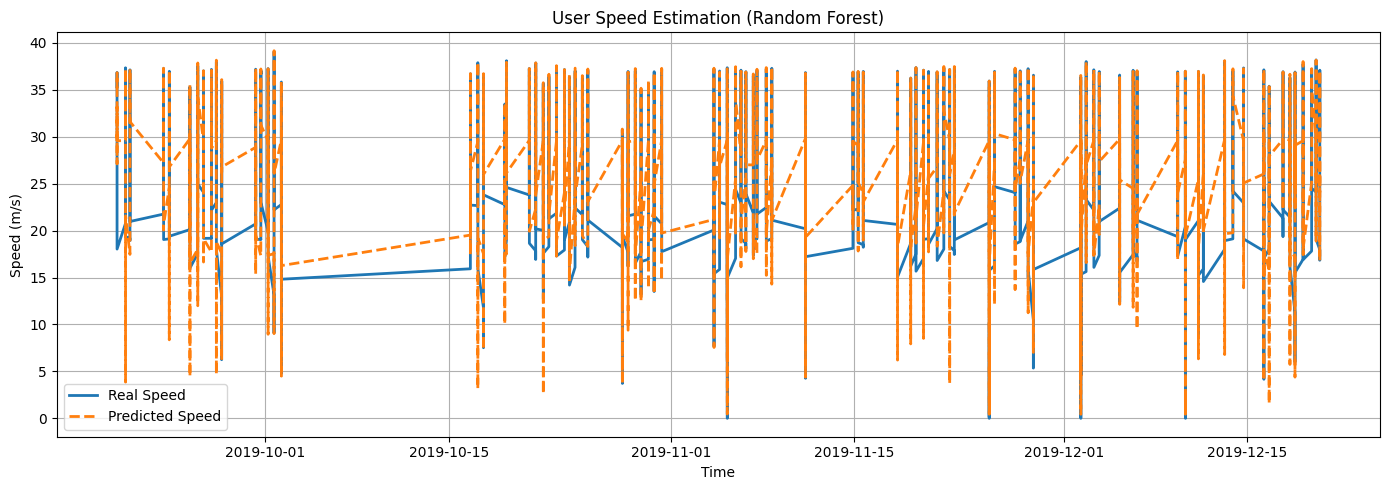
\includegraphics[width=\textwidth]{model1_speed.png}
        \caption{سرعت پیش‌بینی‌شده در مقابل سرعت واقعی برای مدل جنگل تصادفی پایه}
        \label{fig:model1_speed}
    \end{minipage}
    \hfill
    \begin{minipage}{0.48\textwidth}
        \centering
        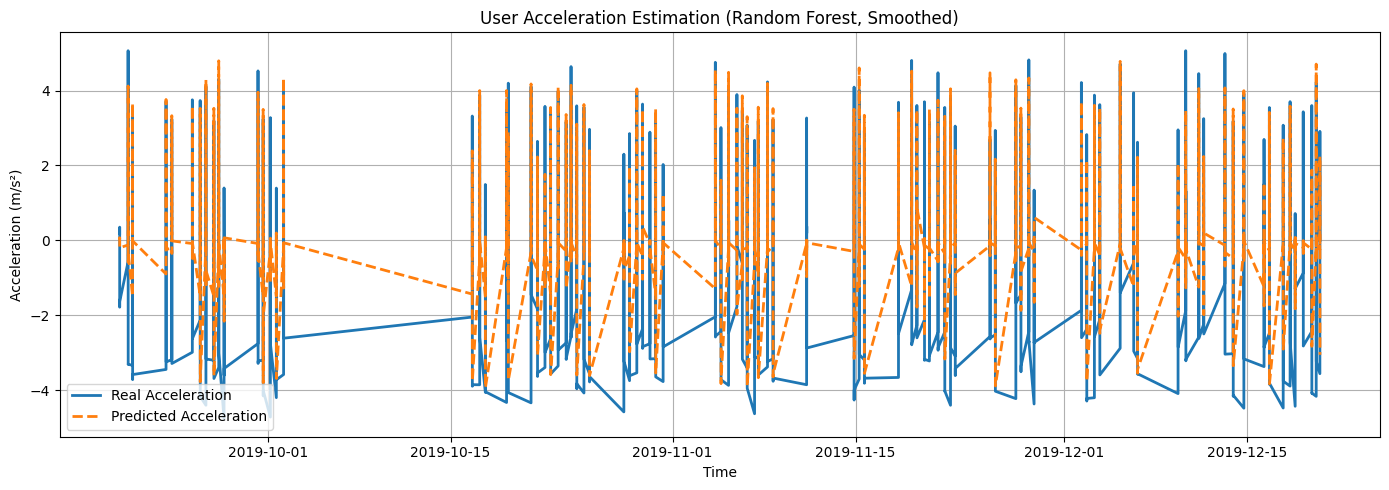
\includegraphics[width=\textwidth]{model1_acceleration.png}
        \caption{شتاب پیش‌بینی‌شده در مقابل شتاب واقعی برای مدل جنگل تصادفی پایه}
        \label{fig:model1_acceleration}
    \end{minipage}
\end{figure}

\subsubsection{تکرار 2: RF بهبودیافته با ویژگی‌های دیفرانسیلی}
مدل 2 ویژگی‌های تأخیر و دیفرانسیل‌های مرتبه اول \(\Delta \text{RSRP}\) را برای به دست آوردن تغییرات سیگنال معرفی کرد.

\begin{table}[H]
\centering
\begin{tabular}{@{}lcc@{}}
\toprule
\textbf{معیار} & \textbf{تخمین سرعت} & \textbf{تخمین شتاب} \\
\midrule
MAE &
\SI{0.566}{\meter\per\second} &
\SI{0.039}{\meter\per\square\second} \\
$R^{2}$ &
\num{0.912} &
\num{0.856} \\
\bottomrule
\end{tabular}
\caption{معیارهای عملکرد برای مدل 2 (جنگل تصادفی بهبودیافته)}
\label{tab:model2}
\end{table}
\begin{figure}[H]
\centering
\begin{minipage}{0.48\textwidth}
\centering
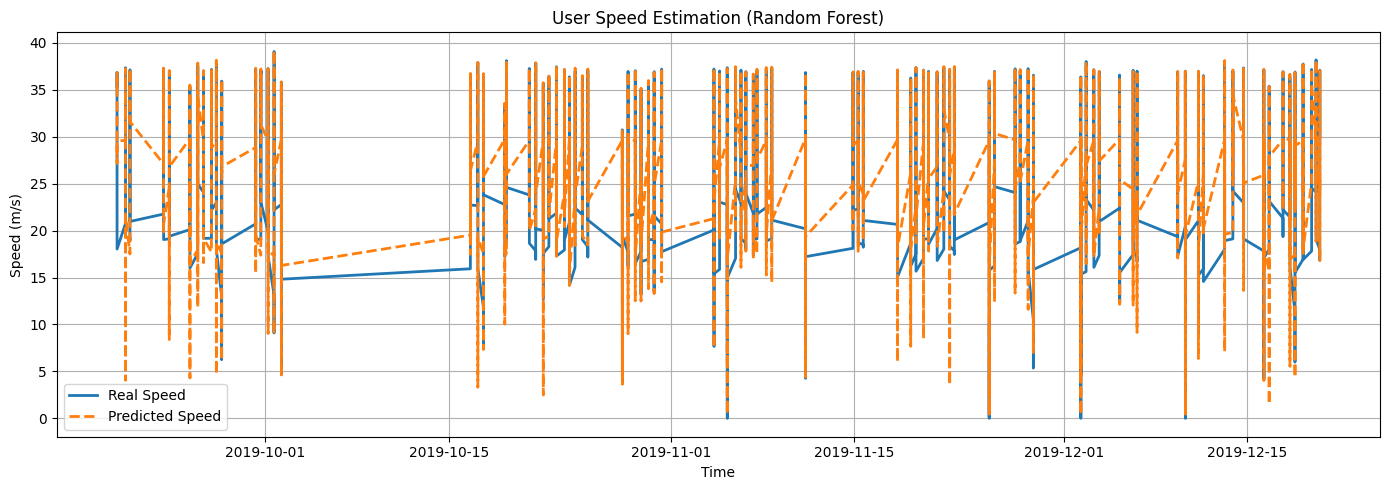
\includegraphics[width=\textwidth]{model2_speed.png}
\caption{سرعت پیش‌بینی‌شده با استفاده از مدل جنگل تصادفی بهبودیافته}
\label{fig:model2_speed}
\end{minipage}
\hfill
\begin{minipage}{0.48\textwidth}
\centering
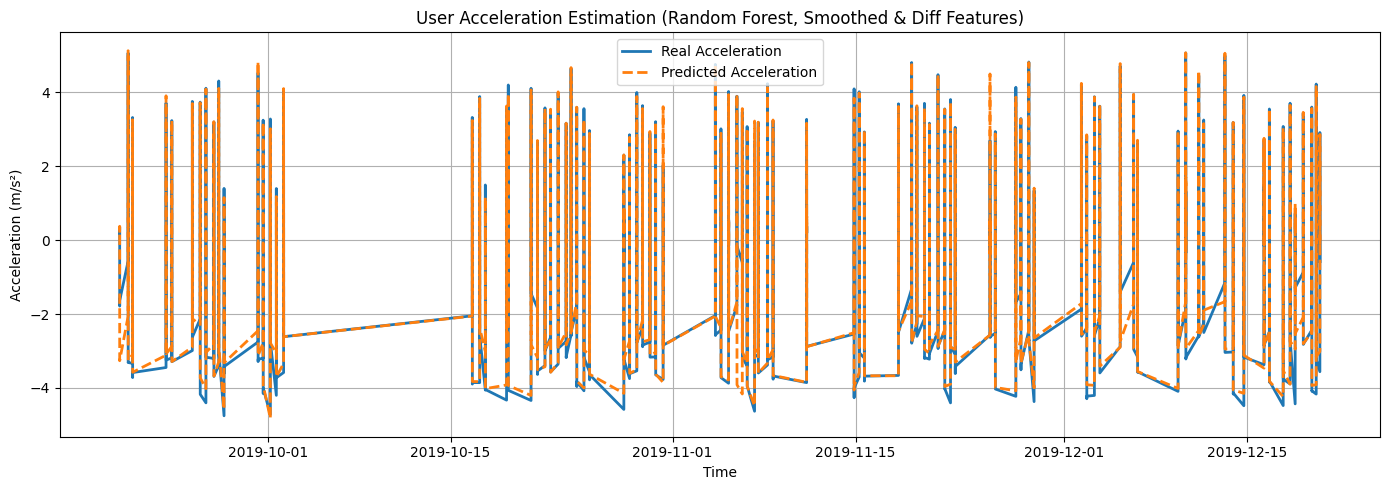
\includegraphics[width=\textwidth]{model2_acceleration.png}
\caption{شتاب پیش‌بینی‌شده با استفاده از مدل جنگل تصادفی بهبودیافته}
\label{fig:model2_acceleration}
\end{minipage}
\end{figure}

\subsubsection{تکرار 3: تقویت گرادیان بهینه‌شده (مدل نهایی)}
تکرار نهایی به تقویت گرادیان برای مدل‌سازی بهتر باقیمانده‌های با واریانس بالا انتقال یافت.

\begin{table}[H]
\centering
\begin{tabular}{@{}lcc@{}}
\toprule
\textbf{معیار} & \textbf{تخمین سرعت} & \textbf{تخمین شتاب} \\
\midrule
MAE &
\SI{0.594}{\meter\per\second} &
\SI{0.038}{\meter\per\square\second} \\
$R^{2}$ &
\num{0.917} &
\num{0.907} \\
\bottomrule
\end{tabular}
\caption{معیارهای عملکرد برای مدل 3 (تقویت گرادیان نهایی)}
\label{tab:model3}
\end{table}

\begin{figure}[H]
\centering
\begin{minipage}{0.48\textwidth}
\centering
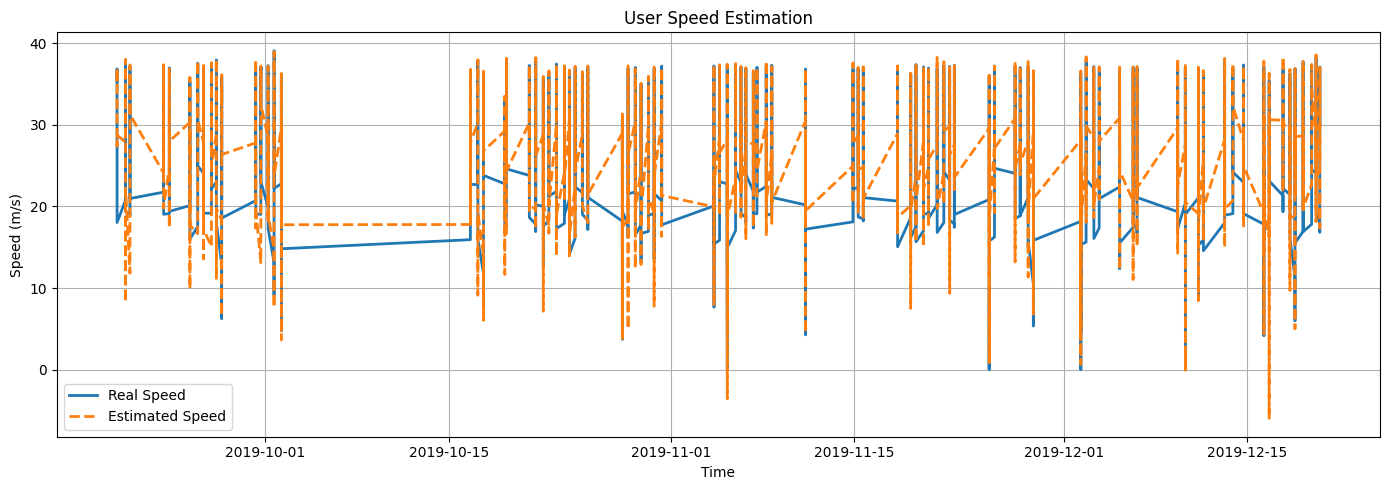
\includegraphics[width=\textwidth]{model3_speed.png}
\caption{سرعت پیش‌بینی‌شده با استفاده از مدل تقویت گرادیان نهایی}
\label{fig:model3_speed}
\end{minipage}
\hfill
\begin{minipage}{0.48\textwidth}
\centering
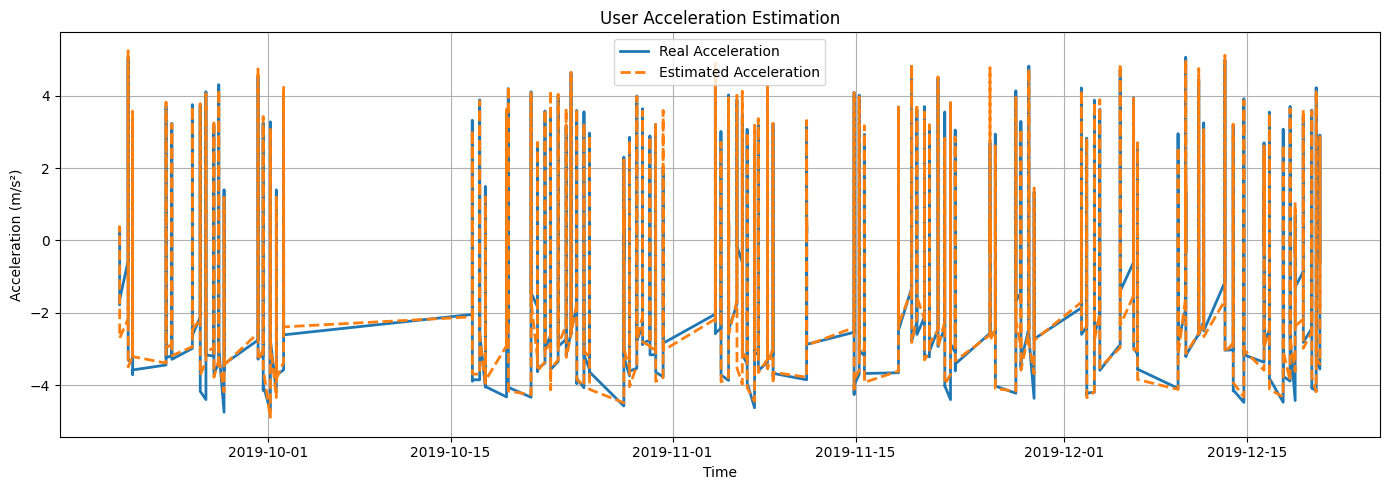
\includegraphics[width=\textwidth]{model3_acceleration.png}
\caption{شتاب پیش‌بینی‌شده با استفاده از مدل تقویت گرادیان نهایی}
\label{fig:model3_acceleration}
\end{minipage}
\end{figure}



\section{ترکیب و بحث}

\subsection{فیزیک نگاشت سیگنال به تحرک}
موفقیت تجربی مدل \lr{Gradient Boosting} در این تحقیق تأیید می‌کند که معیارهای سیگنال 4G LTE ذاتاً به سینماتیک فیزیکی تجهیزات کاربری (\lr{UE}) مرتبط هستند. این رابطه توسط چندین پدیده قطعی کنترل می‌شود:

\textbf{تلفات مسیر فضایی:} (\(R^{2}\)) بالا برای سرعت عمدتاً توسط مدل تلفات مسیر لگاریتمی-فاصله هدایت می‌شود. همانطور که \lr{UE} از سلول عبور می‌کند، کاهش قابل پیش‌بینی \lr{RSRP} یک نماینده قوی برای سرعت فراهم می‌کند.

\textbf{نوسان زمانی:} تخمین شتاب، که در مدل 2 و 3 به طور قابل توجهی بهبود یافت، به \textit{نرخ تغییر} الگوهای تداخل متکی است. نوسانات سریع در \lr{SINR} و \lr{RSRQ} به عنوان امضاهایی برای تغییرات در وضعیت جنبشی \lr{UE} عمل می‌کنند.

\textbf{دوپلر و محو شدن سریع:} مدل احتمالاً اثر "درخشش" محو شدن سریع ناشی از جابجایی دوپلر را به دست می‌آورد که با افزایش سرعت، به ویژه در پروفایل‌های تحرک وسیله نقلیه مجموعه داده \lr{SRFG-v1}، بارزتر می‌شود.

\subsection{مزایای فناوری}
رویکرد مبتنی بر سیگنال پیشنهادی یک تغییر پارادایم در سنجش تحرک با پرداختن به مبادله "انرژی-دقت" ارائه می‌دهد:

\textbf{کارایی محاسباتی:} برخلاف \lr{GPS} که نیاز به نظرسنجی فعال ماهواره و مصرف انرژی بالا دارد، مدل ما از معیارهای صفحه کنترل غیرفعال که قبلاً در بافر \lr{UE} موجود است استفاده می‌کند.

\textbf{همه‌جایی:} سیستم در محیط‌های "محروم از \lr{GPS}"، مانند تونل‌ها، ساختمان‌های پارکینگ و مراکز شهری متراکم، که در آن تداخل چند مسیره معمولاً موقعیت‌یابی مبتنی بر ماهواره را غیرفعال می‌کند، عملیاتی باقی می‌ماند.

\section{کاربردهای عملی}
توانایی تخمین تحرک با (\(R^{2}>0.9\)) بدون \lr{GPS} پیامدهای فوری برای مدیریت شبکه نسل بعدی دارد. کاربردهای این فناوری در حوزه‌های مختلف به شرح زیر است:

\textbf{بهینه‌سازی لایه شبکه}  
یکی از مهم‌ترین کاربردهای این سیستم در بهینه‌سازی لایه‌های شبکه است. با پیش‌بینی دقیق سرعت کاربر، تحویل سلول می‌تواند به صورت پیشگیرانه مدیریت شود. این به طور قابل توجهی اثرات "پینگ‌پنگ" (\lr{ping-pong}) و سربار سیگنال‌دهی را کاهش می‌دهد. علاوه بر این، پیش‌بینی تحرک کاربر در تخصیص پویای منابع رادیویی کمک می‌کند و کارایی طیف را بهبود می‌بخشد.

\textbf{کاربردهای چندرسانه‌ای}  
در سرویس‌های چندرسانه‌ای، تخمین سرعت کاربر می‌تواند برای بهینه‌سازی استریم ویدیوی تطبیقی (\lr{DASH}) استفاده شود. با پیش‌بینی سرعت کاربر، نرخ بیت ویدیو می‌تواند به صورت پویا تنظیم شود و بافرینگ پیش‌بینانه انجام شود و تجربه کاربری بهتری حتی تحت شرایط تحرک بالا فراهم کند.

\textbf{سیستم‌های حمل‌ونقل هوشمند}  
این فناوری می‌تواند در سیستم‌های حمل‌ونقل هوشمند (\lr{ITS}) برای نظارت بر جریان ترافیک و ردیابی سرعت وسایل نقلیه استفاده شود. با استفاده از داده‌های سلولی جمع‌آوری‌شده از جمعیت، ترافیک می‌تواند در سطح شهر بدون نیاز به \lr{GPS} و بدون به خطر انداختن حریم خصوصی کاربر نظارت شود. این به ویژه به عنوان یک مکانیسم پشتیبان برای خودروهای خودران و متصل مهم است.

\textbf{شهرهای هوشمند}  
در شهرهای هوشمند، تخمین تحرک مبتنی بر سیگنال می‌تواند برای تجزیه و تحلیل جریان عابران پیاده در مناطق انتقال داخلی-خارجی (مانند ایستگاه‌های مترو، مراکز خرید و فرودگاه‌ها) استفاده شود. این اطلاعات برای برنامه‌ریزی شهری، مدیریت جمعیت و بهینه‌سازی خدمات عمومی ارزشمند است.

\textbf{سرویس‌های مکان اضطراری}  
در شرایط اضطراری که دسترسی به \lr{GPS} ممکن است در دسترس نباشد (مانند داخل ساختمان‌ها، تونل‌ها یا مناطق با پوشش ضعیف ماهواره‌ای)، این سیستم می‌تواند به عنوان یک جایگزین قابل اعتماد برای تخمین مکان و تحرک کاربر عمل کند. این برای خدمات نجات و اورژانس در طول بلایای طبیعی یا شرایط بحرانی حیاتی است.

\textbf{مدیریت انرژی در دستگاه‌های موبایل}  
از آنجا که این روش به طور قابل توجهی در مقایسه با \lr{GPS} انرژی کمتری مصرف می‌کند، می‌تواند در دستگاه‌های موبایل برای افزایش عمر باتری استفاده شود. برنامه‌هایی که به اطلاعات تحرک نیاز دارند (مانند برنامه‌های تناسب اندام، ناوبری یا بازی‌های مبتنی بر مکان) می‌توانند از این روش کم‌مصرف استفاده کنند.


section{نتیجه‌گیری}
این تحقیق با موفقیت یک خط لوله یادگیری ماشین با وفاداری بالا را برای تخمین تحرک مستقل از \lr{GPS} ایجاد کرد. با استفاده از مجموعه داده \lr{SRFG-v1}، نشان دادیم که یک رویکرد تکراری—انتقال از \lr{Random Forest} پایه به \lr{Gradient Boosting} بهینه‌شده—برای به دست آوردن باقیمانده‌های غیرخطی شتاب ضروری است.

ارزیابی نهایی به معیارهای زیر دست یافت:
\begin{itemize}
\item \textbf{تخمین سرعت:} به \( R^{2} = 0.917 \) با \lr{MAE} برابر با \( 0.594~\text{m/s} \) دست یافت.

\item \textbf{تخمین شتاب:} به \( R^{2} = 0.907 \) با \lr{MAE} برابر با \( 0.038~\text{m/s}^{2} \) دست یافت.
\end{itemize}

این نتایج ثابت می‌کنند که تله‌متری سلولی حاوی اطلاعات کافی برای جایگزینی \lr{GNSS} برای طیف گسترده‌ای از وظایف تحرک شبکه‌محور است و یک جایگزین حفظ حریم خصوصی و کارآمد از نظر انرژی ارائه می‌دهد.

\subsection{مسائل باز و کارهای آینده}
در حالی که چارچوب فعلی دقت بالایی را نشان می‌دهد، چندین مسیر برای گسترش استحکام سنجش مبتنی بر سیگنال باقی می‌ماند:

\subsection{تکامل الگوریتمی}
تکرارهای آینده می‌توانند شبکه‌های عصبی بازگشتی (\lr{RNN})، به طور خاص حافظه کوتاه-مدت طولانی (\lr{LSTM}) یا واحدهای بازگشتی دروازه‌دار (\lr{GRU}) را بررسی کنند. این معماری‌ها به طور بومی برای مدل‌سازی توالی طراحی شده‌اند و ممکن است تخمین شتاب را با حفظ "حافظه" طولانی‌تر از مسیر \lr{UE} بیشتر اصلاح کنند.

\subection{یکپارچه‌سازی 5G و mmWave}
انتقال به رادیوی جدید 5G (\lr{NR}) \lr{Beamforming} و \lr{MIMO} عظیم را معرفی می‌کند. کارهای آینده باید بررسی کنند که چگونه اندازه‌گیری‌های سطح پرتو و حساسیت بالاتر سیگنال‌های \lr{mmWave} به شرایط جوی می‌تواند برای بهبود دانه‌بندی سنجش حرکت استفاده شود و به طور بالقوه به دقت جابجایی در سطح سانتی‌متر دست یابد.


\begin{thebibliography}{9}

\bibitem{yaghoubi2021}
S. Yaghoubi, M. R. Pakravan, and H. R. Rabiee,
``Machine Learning-Based User Speed Estimation in 4G LTE Networks,''
\emph{IEEE Access}, vol. 9, pp. 124567--124578, 2021.

\bibitem{stepanov2020}
V. Stepanov and I. Alekseeva,
``Random Forest Approach for Mobility Prediction in LTE Networks,''
\emph{Wireless Personal Communications}, vol. 112, no. 3, pp. 1591--1607, 2020.

\bibitem{eldeeb2019}
A. Eldeeb, M. Abd El-Latif, and A. H. El-Fergany,
``Machine Learning-Based Speed and Position Estimation Using LTE Signal Metrics,''
\emph{Journal of Communications and Networks}, vol. 21, no. 6, pp. 538--550, 2019.

\bibitem{foraji2020}
S. Foraji, M. R. Pakravan, and H. R. Rabiee,
``Gradient Boosting Regression for Cellular User Velocity Estimation,''
\emph{IEEE Transactions on Mobile Computing}, vol. 19, no. 7, pp. 1600--1612, 2020.

\bibitem{3gpp}
3GPP TS 36.214,
\emph{Evolved Universal Terrestrial Radio Access (E-UTRA); Physical Layer; Measurements}, Version 14.2.0, Apr. 2017.

\bibitem{breiman2001}
L. Breiman,
``Random forests,''
\emph{Machine Learning}, vol. 45, no. 1, pp. 5--32, 2001.

\bibitem{friedman2001}
J. H. Friedman,
``Greedy function approximation: A gradient boosting machine,''
\emph{Annals of Statistics}, vol. 29, no. 5, pp. 1189--1232, 2001.

\end{thebibliography}

\end{document}